% This is text associated with the open textbook "Open Electromagnetics"
% See immediately below for author, date
% This work is licensed under the Creative Commons Attribution-ShareAlike 4.0 International License. (CC BY-SA 4.0) 
% To view a copy of the license, visit http://creativecommons.org/licenses/by-sa/4.0/

%ORB TITLE Spherical Coordinates
%ORB AUTHOR 0        # S.W. Ellingson, Virginia Tech (ellingson@vt.edu)
%ORB DATE 20180703   # yyyymmdd
%ORB ABSTRACT Spherical Coordinates

\label{m0097_Spherical_Coordinates} % <-- Must match name of this file and module directory name.  Don't mess with this!
\index{spherical coordinate system|(}

The spherical coordinate system is defined with respect to the Cartesian system in Figure~\ref{m0097_fSphericalCoordinates}.
The spherical system uses $r$, the distance measured from the origin;\footnote{Note that some textbooks use ``$R$'' in lieu of $r$ for this coordinate.} $\theta$, the angle measured from the $+z$ axis toward the $z=0$ plane; and $\phi$, the angle measured in a plane of constant $z$, identical to $\phi$ in the cylindrical system.
%
\begin{figure}[b!]
\begin{center}
\pdftooltip{{  % note double braces
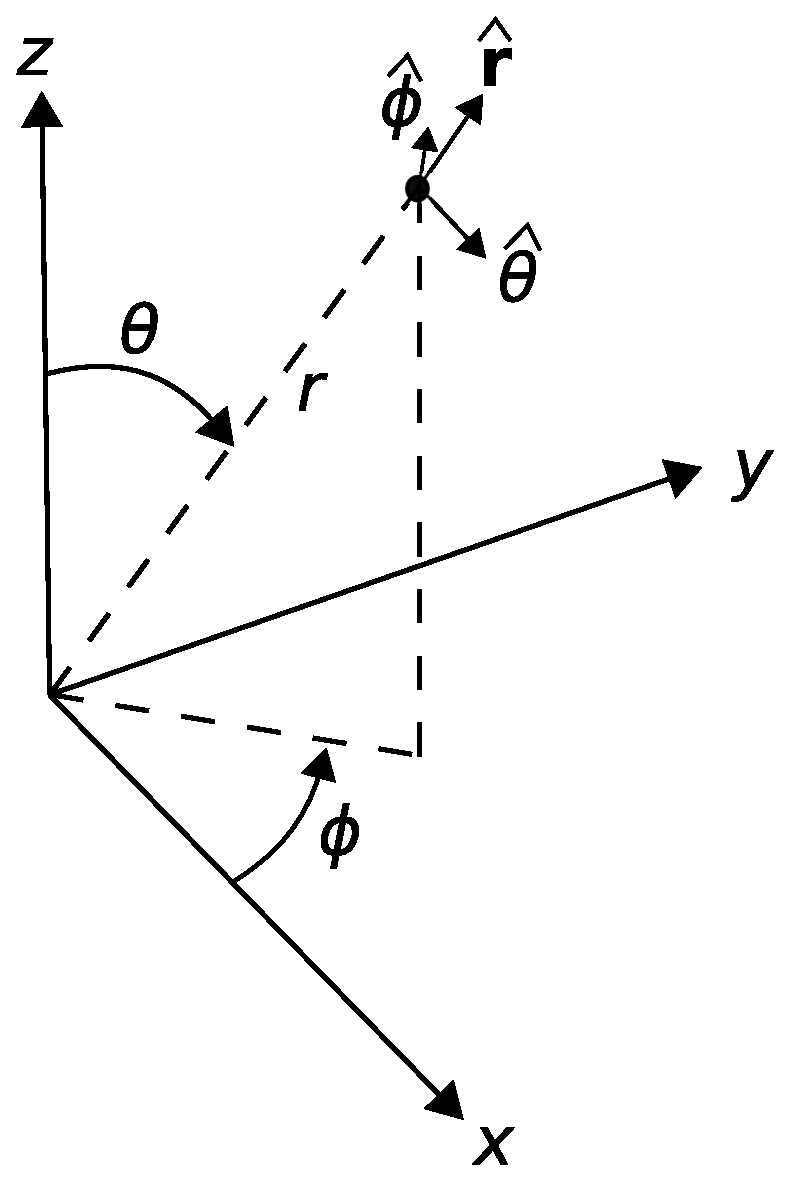
\includegraphics[width=2in]{modules/m0097_fSphericalCoordinates.eps}
% https://commons.wikimedia.org/wiki/File:Spherical_Coordinate_System.svg
}}{Cartesian coordinate system with a point arbitrarily plotted in the positive x, y, and z axes. A dashed line forms an acute triangle with one point at the origin of the Cartesian coordinate system and the top point connected to the arbitrary point with hypotenuse labeled r. The angle from the x-axis to the bottom side of the triangle is labeled phi. The angle from the z-axis to the hypotenuse is labeled theta. From the arbitrary point, vectors labeled phi-hat, r-hat, and theta-hat extend. The phi-hat vector extends parallel to the z-axis. Theta-hat extends parallel to the x-axis. R-hat is perpendicular to phi-hat and theta-hat.}
\end{center} 
\centerline{\scriptsize 
\copyright~\hyperref[m0097_fSphericalCoordinates_Credit]{K.\ Kikkeri} 
\href{https://creativecommons.org/licenses/by-sa/4.0/}{CC BY~SA 4.0} 
} 
\caption{
\label{m0097_fSphericalCoordinates}
Spherical coordinate system and associated basis vectors.
}
\end{figure}

Spherical coordinates are preferred over Cartesian and cylindrical coordinates when the geometry of the problem exhibits spherical symmetry.
For example, in the Cartesian coordinate system, the surface of a sphere concentric with the origin requires all three coordinates ($x$, $y$, and $z$) to describe.
However, this surface can be described using a single constant parameter -- the radius $r$ -- in the spherical coordinate system.
This leads to a dramatic simplification in the mathematics in certain applications.

The basis vectors in the spherical system are $\hat{\bf r}$, $\hat{\bf \theta}$, and $\hat{\bf \phi}$.
As always, the dot product of like basis vectors is equal to one, and the dot product of unlike basis vectors is equal to zero.
For the cross-products, we find:
%
\begin{equation}
\hat{\bf r} \times \hat{\bf \theta} = \hat{\bf \phi}
\end{equation}
%
\begin{equation}
\hat{\bf \theta} \times \hat{\bf \phi} = \hat{\bf r}
\end{equation}
%
\begin{equation}
\hat{\bf \phi} \times \hat{\bf r} = \hat{\bf \theta}
\end{equation}
%
A useful diagram that summarizes these relationships is shown in Figure~\ref{m0097_fSphericalBasisCrossProducts}.
%
\begin{figure}
\begin{center}
\pdftooltip{{  % note double braces
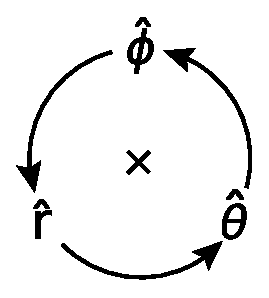
\includegraphics[width=1in]{modules/m0097_fSphericalBasisCrossProducts.eps}
}}{The symbols for r-hat, theta-hat, and phi-hat are arranged in a circle, connected by arrows pointing in a counter-clockwise direction.  A cross product symbol appears in the center of the circle.}
\end{center} 
\caption{\label{m0097_fSphericalBasisCrossProducts}Cross products among basis vectors in the spherical system. (See Figure~\ref{m0006_fCartesianBasisCrossProducts} for instructions on the use of this diagram.)}
\end{figure}

Like the cylindrical system, the spherical system is often less useful than the Cartesian system for identifying absolute and relative positions.
The reason is the same: Basis directions in the spherical system depend on position.
For example, $\hat{\bf r}$ is directed radially outward from the origin, so $\hat{\bf r}=\hat{\bf x}$ for locations along the $x$-axis but $\hat{\bf r}=\hat{\bf y}$ for locations along the $y$ axis and $\hat{\bf r}=\hat{\bf z}$ for locations along the $z$ axis.
Similarly, the directions of $\hat{\bf \theta}$ and $\hat{\bf \phi}$ vary as a function of position.
To overcome this awkwardness, it is common to begin a problem in spherical coordinates, and then to convert to Cartesian coordinates at some later point in the analysis.  
Here are the conversions:
%
\begin{align}
x &= r \cos\phi \sin\theta \label{m0097_es2cx} \\
y &= r \sin\phi \sin\theta \label{m0097_es2cy} \\
z &= r \cos\theta          \label{m0097_es2cz}
\end{align}
%
The conversion from Cartesian to spherical coordinates is as follows:
%
\begin{align}
r      &= \sqrt{x^2+y^2+z^2}      \\
\theta &= \arccos\left(z/r\right) \\
\phi   &= \arctan\left(y,x\right) \\
\end{align}
%
where $\arctan$ is the four-quadrant inverse tangent function.\footnote{Note that this function is available in MATLAB and Octave as {\tt atan2(y,x)}.}
%*** TODO PROBLEM *** \theta in terms of rho and z: 
%*** TODO PROBLEM *** cartesian to spherical conversion problem from page 7 of 3105 notes

Dot products between basis vectors in the spherical and Cartesian systems are summarized in Table~\ref{m0097_tBasisVectorConversion}.
This information can be used to convert between basis vectors in the spherical and Cartesian systems, in the same manner described in Section~\ref{m0096_Cylindrical_Coordinates}; e.g.
%
\begin{equation}
\hat{\bf x} = \hat{\bf r     }\left(\hat{\bf r     }\cdot\hat{\bf x}\right) 
             +\hat{\bf \theta}\left(\hat{\bf \theta}\cdot\hat{\bf x}\right)
             +\hat{\bf \phi  }\left(\hat{\bf \phi  }\cdot\hat{\bf x}\right)
\end{equation}
%
\begin{equation}
\hat{\bf r} = \hat{\bf x}\left(\hat{\bf x}\cdot\hat{\bf r}\right) 
             +\hat{\bf y}\left(\hat{\bf y}\cdot\hat{\bf r}\right)
             +\hat{\bf z}\left(\hat{\bf z}\cdot\hat{\bf r}\right)
\end{equation}
%
and so on.
%*** TODO PROBLEM *** write above explicitly
% 
%Using this table, we find
%%
%\begin{equation}
%\hat{\bf x} = \hat{\bf r}\sin\theta\cos\phi
%             +\hat{\bf \theta}\cos\theta\cos\phi
%             -\hat{\bf \phi}\sin\phi
%%\end{equation}
%%
%\begin{equation}
%\hat{\bf y} = \hat{\bf r}\sin\theta\sin\phi
%             +\hat{\bf \theta}\cos\theta\sin\phi
%             +\hat{\bf \phi}\cos\phi
%\end{equation}
%%
%\begin{equation}
%\hat{\bf z} = \hat{\bf r}\cos\theta
%             -\hat{\bf \theta}\sin\theta
%\end{equation}
%
\begin{table}
\begin{center}
\begin{tabular}{c|ccc}
$\cdot$       & $\hat{\bf r}$ & $\hat{\bf \theta}$ & $\hat{\bf \phi}$ \\
\hline
$\hat{\bf x}$ & $\sin\theta\cos\phi$ & $~\cos\theta\cos\phi$ & $-\sin\phi$ \\
$\hat{\bf y}$ & $\sin\theta\sin\phi$ & $~\cos\theta\sin\phi$ & $~\cos\phi$ \\
$\hat{\bf z}$ & $\cos\theta$         & $-\sin\theta$         & 0 \\
\end{tabular}
\end{center}
\caption{\label{m0097_tBasisVectorConversion}Dot products between basis vectors in the spherical and Cartesian coordinate systems.}
\end{table}

%ORB EXAMPLE
~\\ \begin{example} 
\begin{mdframed}[backgroundcolor=brown!20,linecolor=brown!20]\raggedright
Cartesian to spherical conversion. 
\\~\\
A vector field ${\bf G} = \hat{\bf x}~xz/y$.  Develop an expression for ${\bf G}$ in spherical coordinates.

{\bf Solution:} Simply substitute expressions in terms of spherical coordinates for expressions in terms of Cartesian coordinates. 
Use Table~\ref{m0097_tBasisVectorConversion} and Equations~\ref{m0097_es2cx}--\ref{m0097_es2cz}. 
Making these substitutions and applying a bit of mathematical clean-up afterward, one obtains  
%
\begin{align}
{\bf G} =& \left( \hat{\bf r}\sin\theta\cot\phi + \hat{\bf\phi}\cos\theta\cot\phi - \hat{\bf \phi} \right) \nonumber \\
         & \cdot r\cos\theta\cos\phi
\end{align}

\end{mdframed}\end{example}


%---------------------------------------------------------------------

{\bf Integration Over Length.}  
A differential-length segment of a curve in the spherical system is
%
\begin{equation}
d{\bf l} = \hat{\bf r}~dr + \hat{\bf \theta}~r~d\theta + \hat{\bf \phi}~r\sin\theta~d\phi 
\end{equation}
%
Note that $\theta$ is an angle, as opposed to a distance. The associated distance is $r~d\theta$ in the $\theta$ direction.
Note also that in the $\phi$ direction, distance is $r~d\phi$ in the $z=0$ plane and less by the factor $\sin\theta$ for $z<>0$. 

As always, the integral of a vector field ${\bf A}({\bf r})$ over a curve ${\mathcal C}$ is
%
\begin{equation}
\int_{\mathcal C}{ {\bf A}\cdot d{\bf l} }
\end{equation}
%
To demonstrate line integration in the spherical system, imagine a sphere of radius $a$ centered at the origin with ``poles'' at $z=+a$ and $z=-a$.
Let us calculate the integral of ${\bf A}({\bf r})=\hat{\bf \theta}$, where $\mathcal{C}$ is the arc drawn directly from pole to pole along the surface of the sphere, as shown in Figure~\ref{m0097_fArc}.  In this example, 
$d{\bf l} = \hat{\bf \theta}~a~d\theta$ 
since $r=a$ and $\phi$ (which could be any value) are both constant along ${\mathcal C}$.  
Subsequently, ${\bf A}\cdot d{\bf l}=a~d\theta$ and the above integral is
%
\begin{equation}
\int_{0}^{\pi}{ a~d\theta } = \pi a
\end{equation}
%
i.e., half the circumference of the sphere, as expected.
%
\begin{figure}
\begin{center}
\pdftooltip{{  % note double braces
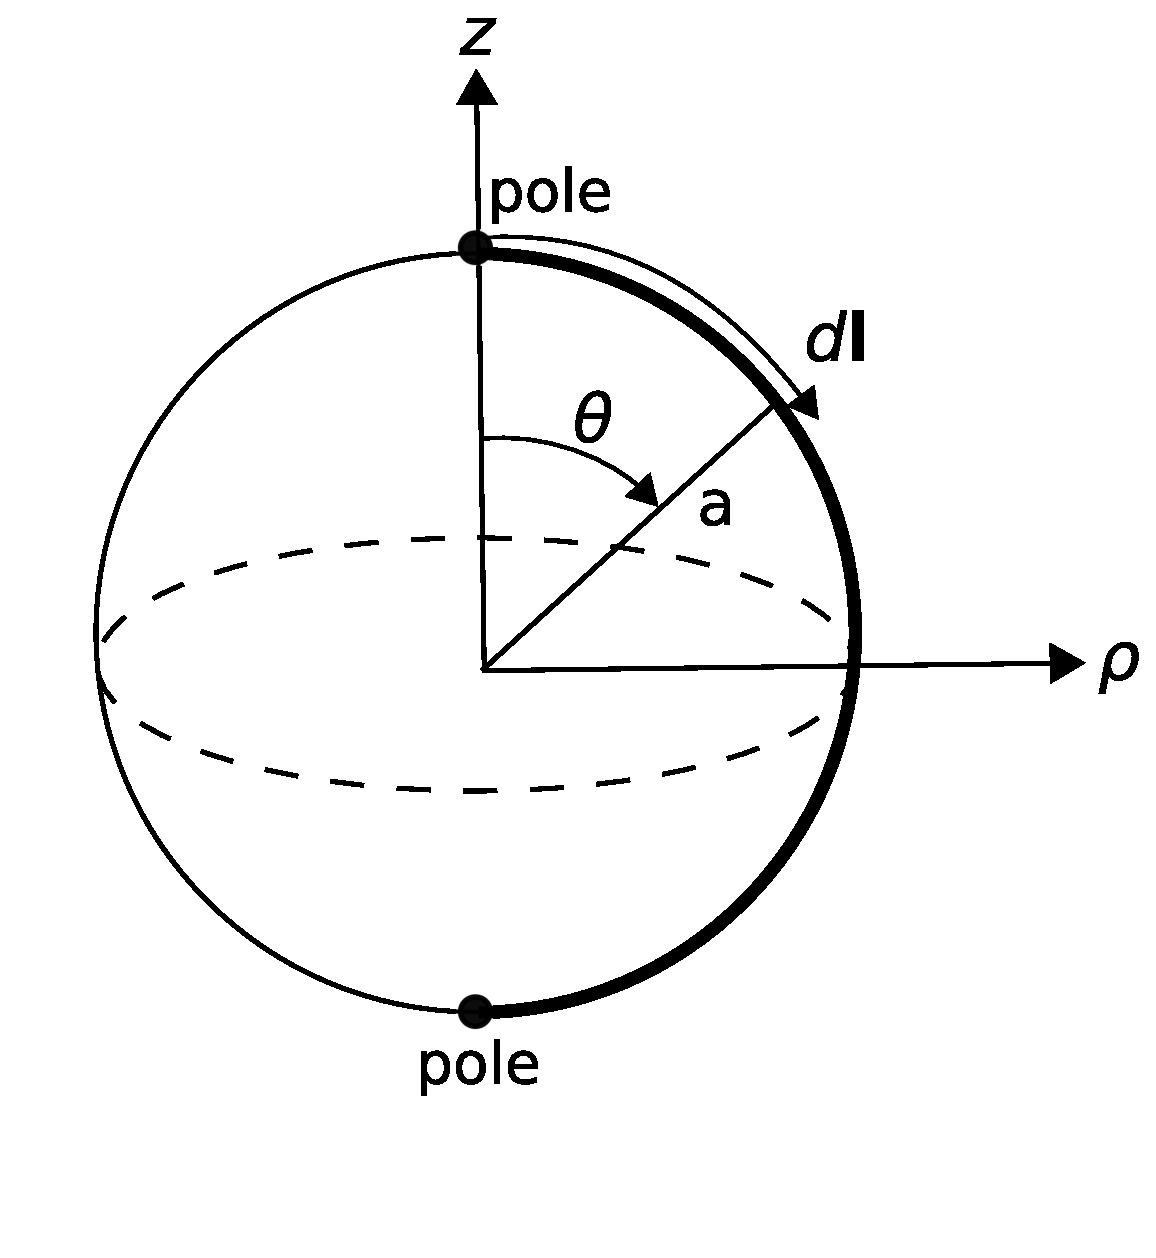
\includegraphics[width=2in]{modules/m0097_fArc.eps}
% https://commons.wikimedia.org/wiki/File:M0097_fArc.svg
}}{A three dimensional sphere centered at the intersection of the rho and z axes. The radius (a) shown at unspecified angle in the first quadrant of the sphere. The north and south poles of the sphere are labeled, and the circumference between them is bolded. From the north pole to the radius (a) is a vector labeled dl. The angle from the z-axis to the radius (a) is labeled theta. }
\end{center} 
\centerline{\scriptsize 
\copyright~\hyperref[m0097_fArc_Credit]{K.\ Kikkeri} 
\href{https://creativecommons.org/licenses/by-sa/4.0/}{CC BY~SA 4.0} 
} 
\caption{
\label{m0097_fArc}
Example in spherical coordinates: Pole-to-pole distance on a sphere.
}
\end{figure}

Note that the spherical system is an appropriate choice for this example because the problem can be expressed with the minimum number of varying coordinates in the spherical system.
If we had attempted this problem in the Cartesian system, we would find that both $z$ and either $x$ or $y$ (or all three) vary over ${\mathcal C}$ and in a relatively complex way. 

{\bf Integration Over Area.}  
Now we ask the question,
what is the integral of some vector field ${\bf A}$ over the surface ${\mathcal S}$ of a sphere of radius $a$ centered on the origin?
This is shown in Figure~\ref{m0097_fSphereArea}.
The differential surface vector in this case is
%
\begin{equation}
d{\bf s} = \hat{\bf r}~\left( r~d\theta \right) \left( r\sin\theta~d\phi \right) = \hat{\bf r}~r^2\sin\theta~d\theta~d\phi  
\end{equation}
%
As always, the direction is normal to the surface and in the direction associated with positive flux.
\index{flux}
The quantities in parentheses are the distances associated with varying $\theta$ and $\phi$, respectively.
In general, the integral over a surface is
%
\begin{equation}
\int_{\mathcal S} {\bf A}\cdot d{\bf s}
\end{equation}
%
In this case, let's consider ${\bf A}=\hat{\bf r}$; in this case ${\bf A}\cdot d{\bf s} = a^2~\sin\theta~d\theta~d\phi$ and the integral becomes
%
\begin{equation}
\begin{split}
\int_{0}^{\pi}\int_{0}^{2\pi} a^2~\sin\theta~d\theta~d\phi &= a^2 \left( \int_{0}^{\pi} \sin\theta d\theta \right) \left( \int_{0}^{2\pi} d\phi \right) \\
                                                           &= a^2 \left( 2 \right) \left( 2\pi \right) \\
                                                           &= 4\pi a^2
\end{split}
\end{equation}
%
which we recognize as the area of the sphere, as expected.
The corresponding calculation in the Cartesian or cylindrical systems is quite difficult in comparison.
%
\begin{figure}
\begin{center}
\pdftooltip{{  % note double braces
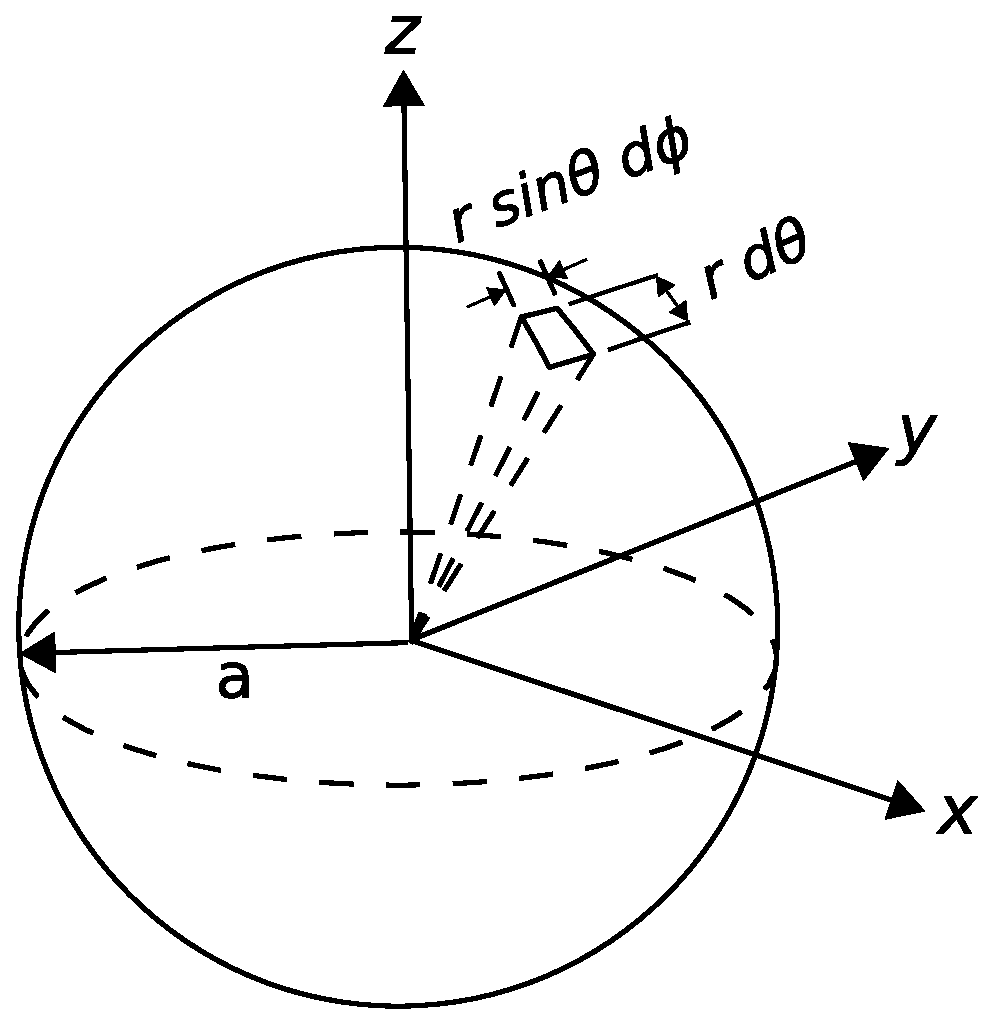
\includegraphics[width=2in]{modules/m0097_fSphereArea.eps}
% https://commons.wikimedia.org/wiki/File:M0097_fSphereArea.svg
}}{A three dimensional sphere lies on a x, y, z axis, with its center at the origin. The radius is labeled a. A square is projected on the surface from the origin, with dashed lines indicating the projection. The width of the box is labeled r * sin(theta) * d phi, and the height of the box is labeled r * d theta.}
\end{center} 
\centerline{\scriptsize 
\copyright~\hyperref[m0097_fSphereArea_Credit]{K.\ Kikkeri} 
\href{https://creativecommons.org/licenses/by-sa/4.0/}{CC BY~SA 4.0} 
} 
\caption{
\label{m0097_fSphereArea}
Example in spherical coordinates: The area of a sphere.
}
\end{figure}

%%% TODO
%~\\ \begin{example} 
%\begin{mdframed}[backgroundcolor=green!20] 
%Flux Through a Spherical Surface. 
%\end{mdframed}
%{\color{red}uniform flux in cartesian direction gives zero flux through sphere but non-zero flux through a half-sphere.}
%\centerline{\rule{2in}{1pt}} \end{example}


%---------------------------------------------------------------------

{\bf Integration Over Volume.}  
The differential volume element in the spherical system is
%
\begin{equation}
dv ~=~ dr \left(r d\theta \right) \left( r \sin\theta d\phi \right) ~=~ r^2 dr~\sin\theta~d\theta~d\phi 
\end{equation}

For example, if $A({\bf r})=1$ and the volume $\mathcal{V}$ is a sphere of radius $a$ centered on the origin, then 
%
\begin{equation}
\begin{split}
\int_{\mathcal V} A({\bf r})~dv  &= \int_0^a \int_0^{\pi} \int_0^{2\pi}  r^2 dr~\sin\theta~d\theta~d\phi \\
                                 &= \left(\int_0^a r^2 dr \right)  \left( \int_0^{\pi} \sin\theta~d\theta \right)  \left( \int_0^{2\pi} d\phi \right) \\
                                 &= \left( \frac{1}{3} a^3 \right)  \left( 2 \right)  \left(  2\pi \right) \\
                                 &= \frac{4}{3}\pi a^3 
\end{split}
\end{equation} 
%
which is the volume of a sphere. 

%%%%%%%%%%%%%%%%%%%%%%%%%%%%%%%%%%%%

{\bf Additional Reading:}
\begin{itemize}
\item ``\href{https://en.wikipedia.org/wiki/Spherical_coordinate_system}{Spherical coordinate system}'' on Wikipedia.
\end{itemize}

\index{spherical coordinate system|)}
